\documentclass[12pt,fleqn,a4paper]{mybook} %Final!!!
%\documentclass[11pt,fleqn,a4paper,draft]{mybook} %DRAFT - highlights overflow, leaves out images

%\usepackage{microtype}
\usepackage[slovak]{babel}
\usepackage[utf8]{inputenc}
\usepackage[T1]{fontenc}

\usepackage{mathtools}  					
\usepackage{graphicx}
\usepackage{subfigure}
\usepackage{enumerate}
\usepackage{etoolbox}                       %Problematic URL in reference
\apptocmd{\sloppy}{\hbadness 10000\relax}{}{}%Removes badness warnings
%This is to remove warnings resulting by otherwise OK URL's
\usepackage[hyphens]{url}
\usepackage{notes}


\usepackage[left=25mm,right=25mm,top=25mm,bottom=25mm,paperwidth=210mm,paperheight=297mm,includehead]{geometry}

\usepackage{titlesec}
\titleformat{\chapter}[hang]{\normalfont\huge\bfseries}{\thechapter}{1em}{}


\DeclarePairedDelimiter{\diagpars}{(}{)}
\newcommand{\diag}{\operatorname{diag}\diagpars}

\let\oldhat\hat
\renewcommand{\vec}[1]{\boldsymbol{\mathbf{#1}}}
%\renewcommand{\hat}[1]{\oldhat{\boldsymbol{\mathbf{#1}}}}


\usepackage{amsthm}
\usepackage{etoolbox}% http://ctan.org/pkg/etoolbo
\theoremstyle{definition}
\newtheorem{exmp}{Pr\'{i}klad}[chapter]
\AtEndEnvironment{exmp}{\null\hfill\qedsymbol}

\usepackage{listings,color} 			    %To list Matlab code
\definecolor{mygrey}{gray}{0.5}	        %Define a gray color
\lstset{
basicstyle=\ttfamily,
numbers=none,
commentstyle=\color{mygrey},
breaklines=true,
}
%extended Matlab language
\lstdefinelanguage{exMatlab}[]{Matlab}      %Defining expanded Matlab
{morekeywords={rng,pyulear,plot,hold,randn,filter,length,abs,periodogram,fft,sin,randn,xcorr,fminsearch,dlqr,predmodelqp,dlyap,ones,linprog,quadprog,optimset,qpOASES,qpOASES_sequence,sysStruct,probStruct,mpt_control,volume,hull,extreme,mpt_exportc,mpt_getInput,sdpvar,blkdiag,sdpsettings,solvesdp,geomean,double},
sensitive=true,
alsoletter={_}
}

 

\pagestyle{empty}

\begin{document}
%%%%%%% Zaciaatok %%%%%%%%
\renewcommand\thepage{\roman{page}}
\pagenumbering{roman}
\thispagestyle{empty}

\noindent \begin{center}
\textbf{{\large{}SLOVENSKÁ TECHNICKÁ UNIVERZITA V BRATISLAVE}}\\
\textbf{{\large{}STROJNÍCKA FAKULTA}}\textbf{\large{} }\\
\vspace{3cm}
\par\end{center}

\noindent \begin{center}
\vspace{3cm}
\par\end{center}



\begin{center}
\textbf{\textsc{\Large{}NÁZOV ZÁVEREČNEJ PRÁCE}}\\
\par\end{center}{\Large \par}

\begin{center}
\textbf{\large{}Bakalárska / Diplomová / Dizertačná práca}\\
\par\end{center}{\large \par}

\begin{center}
{\large{}SjF-12345-67890}\\
\par\end{center}{\large \par}



\vfill
\noindent \textbf{\large{}2018} \hfill \textbf{\large{}Bc. Jožko Mrkvička}
\cleardoublepage

\thispagestyle{empty}

\noindent \begin{center}
\textbf{{\large{}SLOVENSKÁ TECHNICKÁ UNIVERZITA V BRATISLAVE}}\\
\textbf{{\large{}STROJNÍCKA FAKULTA}}\textbf{\large{} }\\
\vspace{3cm}
\par\end{center}

\noindent \begin{center}
\vspace{3cm}
\par\end{center}



\begin{center}
\textbf{\textsc{\Large{}NÁZOV ZÁVEREČNEJ PRÁCE}}\\
\par\end{center}{\Large \par}

\begin{center}
\textbf{\large{}Typ záverečnej práce}\\
\par\end{center}{\large \par}

\begin{center}
{\large{}SjF-12345-67890}\\
\end{center}


\vfill
\begin{flushleft}
$\begin{array}{ll}
\text{Študijný odbor:}&\text{Automatizácia strojov a procesov}\\
\text{Študijný program:}&\text{5.2.14 automatizácia}\\
\text{Školiace pracovisko:}&\text{Ústav automatizácie, merania a aplikovanej informatiky}\\
\text{Vedúci záverečnej práce:}&\text{doc. Ing. Gergely Takács, PhD.}\\
\text{Konzultant:}&\text{Ing. František Mrkvička, PhD.}\\
\end{array}$
\end{flushleft}
\vspace{0.5cm}
\noindent \textbf{\large{}Bratislava, 2018} \hfill \textbf{\large{}Jožko Mrkvička}
\cleardoublepage

Tu je zaviazan� zadanie z�vere�nej pr�ce (v jednom odovzdanom v�tla�ku origin�l zadania, v �al��ch v�tla�koch k�pie zadania).

\cleardoublepage 

	

\null
\vfill
\noindent
\section*{Čestné prehlásenie}

Vyhlasujem, že som záverečnú prácu vypracoval(a) samostatne s použitím uvedenej literatúry.\\

\noindent Bratislava, 20. mája 2018 \hfill $\begin{array}{rl}
                                          &\text{..................................}\\
                                          &\text{Vlastnoručný podpis}\\
                                           \end{array}$
\cleardoublepage


	

\null
\vfill
\noindent
Na tomto mieste môže byť poďakovania napr. vedúcemu diplomovej práce, resp. konzultantom, za pripomienky a odbornú pomoc pri vypracovaní diplomovej práce. Vzor: Ďakujem vedúcemu diplomovej práce, doc. Ing. Jozefovi Jazvečíkovi, PhD., za odbornú pomoc pri vypracovaní diplomovej práce. Chcem poďakovať aj konzultantovi diplomovej práce, Ing. Jánovi Čerešničkovi, za pomoc a pripomienky pri spracovaní nameraných hodnôt.\\

\noindent Bratislava, 20. mája 2018 \hfill Bc. Jožko Mrkvička
\cleardoublepage 


	


\noindent
\textbf{Názov práce:} Meranie sily pomocou tenzometrov\\
\textbf{K¾úèové slová: } (2 až 6 k¾úèových slov) meranie sily, tenzometer, neistota merania, Wheatstonov mostík\\
\textbf{Abstrakt: } (v rozsahu 800 až 900 znakov vrátane medzier) Lorem ipsum dolor sit amet, consectetur adipiscing elit. Donec id scelerisque tortor. Aliquam pretium est metus, at faucibus urna venenatis id. Suspendisse nec sodales leo, in vulputate lacus. Curabitur semper sem eros, a elementum dui accumsan ut. Nunc sit amet arcu mauris. Quisque porttitor nisl a lectus scelerisque, eu pharetra lectus cursus. Etiam volutpat lacus et lorem ornare, eget semper neque bibendum. Cras a iaculis nibh, lacinia sodales diam. Aenean a tempus ante. Proin at eros at dolor volutpat rhoncus. Vivamus ac suscipit turpis. Donec ut ultricies est. Fusce congue sagittis libero ac feugiat. Duis tempus enim in enim malesuada, et vehicula mauris tincidunt. Nullam imperdiet massa nec feugiat convallis. Nunc pellentesque urna quis magna euismod, eu commodo ex aliquam. Ut nullam.\\

\noindent
\textbf{Title:} Force measurement by strain gauges\\
\textbf{Keywords: } (2 až 6 k¾úèových slov) force measurement, strain gauge, measurement uncertainty, Wheatstone bridge\\
\textbf{Abstract: } (v rozsahu 800 až 900 znakov vrátane medzier) Lorem ipsum dolor sit amet, consectetur adipiscing elit. Donec id scelerisque tortor. Aliquam pretium est metus, at faucibus urna venenatis id. Suspendisse nec sodales leo, in vulputate lacus. Curabitur semper sem eros, a elementum dui accumsan ut. Nunc sit amet arcu mauris. Quisque porttitor nisl a lectus scelerisque, eu pharetra lectus cursus. Etiam volutpat lacus et lorem ornare, eget semper neque bibendum. Cras a iaculis nibh, lacinia sodales diam. Aenean a tempus ante. Proin at eros at dolor volutpat rhoncus. Vivamus ac suscipit turpis. Donec ut ultricies est. Fusce congue sagittis libero ac feugiat. Duis tempus enim in enim malesuada, et vehicula mauris tincidunt. Nullam imperdiet massa nec feugiat convallis. Nunc pellentesque urna quis magna euismod, eu commodo ex aliquam. Ut  nullam.
\cleardoublepage 

\chapter*{Predhovor}
\thispagestyle{empty}

Predhovor je nepovinnou n�le�itos�ou z�vere�nej pr�ce. V predhovore autor pr�ce uvedie z�kladn� charakteristiky svojej z�vere�nej pr�ce a okolnosti jej vzniku. Vysvetl� d�vody, ktor� ho viedli k vo�be t�my, cie� a ��el pr�ce a stru�ne informuje o hlavn�ch met�dach, ktor� pri spracovan� z�vere�nej pr�ce pou�il.

\cleardoublepage


\tableofcontents
\thispagestyle{empty}
\cleardoublepage

%%%%%% Jednotlive kapitoly %%%%%%%%%
\pagestyle{plain}
\pagenumbering{arabic}
\setcounter{page}{1}

\chapter*{�vod}
\addcontentsline{toc}{chapter}{�vod}

V �vode autor podrobnej�ie ako v predhovore, pritom v�sti�ne a kr�tko charakterizuje stav poznania alebo praxe v �pecifickej oblasti, ktor� je predmetom z�vere�nej pr�ce. Autor presnej�ie ako v predhovore vysvetl� ciele pr�ce, jej zameranie, pou�it� met�dy a stru�ne objasn� vz�ah pr�ce k in�m pr�cam podobn�ho zamerania. V �vode netreba zach�dza� hlb�ie do te�rie. Netreba podrobne opisova� met�dy, experiment�lne v�sledky, ani opakova� z�very pr�padne odpor��ania.
�vod za��na na novej strane.

\chapter{Z�kladn� triky v LaTeX}
\label{jablka}

\section{Bibliografick� cit�cie}

Citova� m��eme nasledovne \cite{Eykhoff84}. Ak chceme citova� viacero autorov, tak m��eme to robi� naraz \cite{Fontes00,Eykhoff84}. Databazu citovanych dokumentov piseme do suboru *.bib. V�etky typy dokumentov (kniha, �l�nok etc.) m� svoju vlastn� kateg�riu. Autora publik�cie m��eme aj nap�sa�, napr�klad �e v pr�ci Qin a Badgwell \cite{Qin99} dok�zali �e. Cit�cia je s��as�ou vety, m��eme to kombinova� do vety \cite{Karny80} alebo d�va� pred bodkou na koniec \cite{Far90}.

\section{Obr�zky}

Obr�zky m��eme d�va� do textu nasledovne. A potom jednoducho m��eme odvola� na obr�zok pomocou Obr. \ref{OBRAZOK 1.1}.
%************ OBRAZOK **************
\begin{figure}[!tbh]
\centering
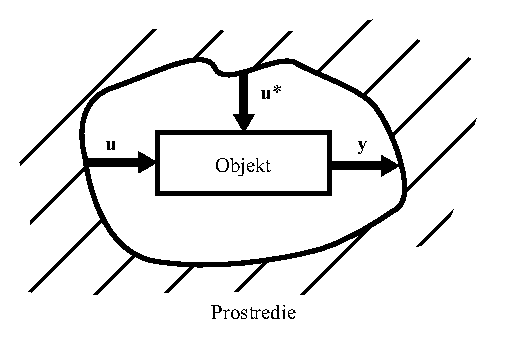
\includegraphics[width=80mm]{obr/OBRAZOK1_1.eps}
\caption{Spojenie objektu s prostred�m}\label{OBRAZOK 1.1}
\end{figure}
%************ KONIEC **************

\section{Odvol�vky na �asti pr�ce}
\label{hrusky}

Kapitolu, podkapitolu alebo podobn� veci ozna��me pr�kazom "label", a nasledovne na nich odvol�me pr�kazom "ref". Napr�klad v Kap. \ref{jablka} sme odvodili ...

\section{Matematika}

Vzorce m��eme pod�a potreby priamo p�sa� do textu, napr�klad: ��seln� postupnos� - mno�ina ��sel $\vec{R} \{a_m, a_{m+1}, ...\}
= \{a_m\}_{m = n}^\infty$, respekt�ve to o��slova� a p�sa� do samostatn�ho riadku napr�klad pomocou
  \begin{align}
  \label{mojarovnica}
    E_0 &= mc^2                              \\
    E &= \frac{mc^2}{\sqrt{1-\frac{v^2}{c^2}}}
  \end{align}
kde potom m��eme odvol�va� na rovnicu pomocou Rov. \eqref{mojarovnica}. Namiesto pr�kazu align, m��eme pou��va� aj eqnarray.


\section{Vymenovanie, ��slovanie}

Z h�adiska sp�sobu, ak�m tvor�me matematick� model, m��eme pri identifik�cii v z�sade postupova� dvoma odli�n�mi sp�sobmi:
\begin{itemize}
\item analyticky, t.j. matematicko - fyzik�lnou anal�zou vlastnost� objektu,
\item experiment�lne.
\end{itemize}
Ka�d� z t�chto sp�sobov m� svoje prednosti a nev�hody.

\begin{enumerate}
  \item Vo�ba triedy oper�torov $S$, na ktorej sa h�ad� vlastn� rie�enie. Ur�enie triedy z�vis� predov�etk�m od objemu apri�rnej inform�cie a znalost� o objekte, mus� v�ak re�pektova� ciele a po�iadavky synt�zy riadenia a ekonomick� ot�zky spojen� s identifik�ciou.
  \item Vo�ba vhodnej stratovej funkcie a na jej b�ze definovanej ��elovej funkcie. Naj�astej�ie s� pou��van� kvadratick� ��elov� funkcie.
  \item V�ber vhodn�ho algoritmu pre rie�enie �lohy identifik�cie, t.j. optimaliza�nej �lohy.
\end{enumerate}

\section{Po��ta�ov� program}

Po��ta�ov� program m��eme jednoducho vlo�i� do textu pomocou
\lstset{language=exMatlab}
\begin{lstlisting}
N=1024;              % Pocet vzoriek
f1=1;                % Frekvencia harmonickeho signalu
FS=200;              % Frekvencia vzorkovania
n=0:N-1;             % Poradove cisla vzorky
x=sin(2*pi*f1*n/FS); % Generujeme signal, x(n)
[Rxx,Tau]=xcorr(x);  % Odhad autokorelacnej funkcie
\end{lstlisting}
Jazyk programu vieme ur�i� my, napr�klad Matlab tu je roz��ren� o extra pr�kazy.


\section{Pr�klad}

Ak chceme uvies� in�truk�n� pr�klad, potom m�me
\begin{exmp}
Jo�ko m� 5 mel�nov, vypo��tajte hmotnos� Slnka.
\end{exmp}
kde pr�klad je ukon�en� znamienkom QED (�tvorec).

\section{Tabu�ky}

Toto je pr�klad tabu�ky:
\begin{table}[!h]
\centering
\caption{Zoradenie met�d na z�klade objemu apri�rnych znalost�}
\begin{tabular}{ |l|c|c|c| }
  \hline
  \parbox[c]{3.5cm}{Met�da} & Kovariancia & \parbox[c]{3cm}{Hustota\\pravdepodobnosti}& Apri�rna hustota\\ [0.2cm] \hline
  \parbox[c]{3.5cm}{Najmen�ie �tvorce} & Nie & Nie & Nie \\ [0.2cm] \hline
  \parbox[c]{3.5cm}{Najmen�ie �tvorce,\\Markov odhad}& �no & Nie & Nie \\ [0.2cm]   \hline
  \parbox[c]{3.5cm}{Maxim�lna\\vierohodnos�}& �no & �no & Nie \\ [0.2cm] \hline
  \parbox[c]{3.5cm}{Bayesovsk� met�dy} & �no & �no & �no \\ [0.2cm] \hline
\end{tabular}
    \label{TABULKA_3_1}
\end{table}

Na tabu�ky taktie� m��eme odvol�va� pomocou Tab. \ref{TABULKA_3_1}. Tabu�ky taktie� maj� popis, d�vame to nad tabu�kou.






\chapter{Ďalšie kapitoly}
\label{kap:3}
Každá kapitola začína na novej strane. Autor rieši zadanú problematiku. Na základe analýzy problému ponúka vlastné riešenia.

\section{Podkapitola}
\label{kap:1.1}

Podkapitoly záverečnej práce majú za úlohu členenie textu práce na dosiahnutie čo naj-väčšej prehľadnosti. Podkapitol môže byť viac, v ich názvoch sa používa desatinné číslovanie. 
%[...]
\chapter{Záver}

Táto časť diplomovej práce je povinná. Autor práce uvedie zhodnotenie riešenia, jeho výhody resp. nevýhody, použitie výsledkov, ďalšie možnosti a podobne.  Môže aj načrtnúť iný spôsob riešenia úloh, resp. uvedie, prečo postupoval uvedeným spôsobom.


%%%%%%% Koniec %%%%%%%%
\bibliographystyle{abbrv}
\addcontentsline{toc}{chapter}{Literat\'{u}ra}
\bibliography{bibliog}
\end{document} 
